\section{Analytical Geometry}

In this section, we will cover the topics for the geometry of \(\mathbb{R}^2\) and \(\mathbb{R}^3\).
An maybe also in higher dimensions.

\subsection{Vectors and Points}
In analytical geometry, points and vectors are the basic elements.

A point in \(\mathbb{R}^3\) is represented as \(\vec{P} = \begin{pmatrix} x \\ y \\ z \end{pmatrix}\).
Or as \((x_1, x_2, \cdots , x_n)\).

A vector is an object with direction and magnitude (in this case), also represented as \(\vec{v} = \begin{pmatrix} v_x \\ v_y \\ v_z \end{pmatrix}\).

Or as \((x_1, x_2, \cdots , x_n)^{T}\).

\subsection{Vector Addition and Scalar Multiplication}
Given two vectors \(\vec{a}\) and \(\vec{b}\):
\[
	\vec{a} \pm  \vec{b} = \begin{pmatrix} a_x \\ a_y \end{pmatrix} \pm \begin{pmatrix} b_x \\ b_y \end{pmatrix} = \begin{pmatrix} a_x \pm b_x \\ a_y \pm b_y \end{pmatrix}
\]

For a scalar \(\lambda\) and vector \(\vec{a}\):
\[
	\lambda \vec{a} = \lambda \begin{pmatrix} a_x \\ a_y \end{pmatrix} = \begin{pmatrix} \lambda a_x \\ \lambda a_y \end{pmatrix}
\]

\begin{figure}[h!]
	\centering
	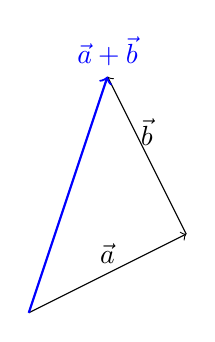
\begin{tikzpicture}
		\draw[->] (0,0) -- (2,1) node[midway, above] {\(\vec{a}\)};
		\draw[->] (2,1) -- (1,3) node[midway, above] {\(\vec{b}\)};
		\draw[->, thick, blue] (0,0) -- (1,3) node[above, above] {\(\vec{a} + \vec{b}\)};
	\end{tikzpicture}
	\caption{Vector addition: \(\vec{a} + \vec{b}\)}
\end{figure}

\subsection{Equation of a Line}
A line is defined by a point \(\vec{P}\) and a direction vector \(\vec{v}\):
\[
	\vec{r}(t) = \vec{P} + t\vec{v}, \quad t \in \mathbb{R}
\]

\subsection{Equation of a Plane}
A plane is defined by a point \(\vec{P}\) and a normal vector \(\vec{n}\):
\[
	P: \vec{x} = \vec{s} + \lambda_1 \vec{v_1} + \lambda_2 \vec{v_2}
\]
\subsection{Scalar (Dot) Product}
The scalar product of vectors \(\vec{a}\) and \(\vec{b}\) is a function \(\langle x, y\rangle :=V \times V \rightarrow \mathbb{K}\)
with the following properties:

\(\forall \vec{a}, \vec{b} \in V\):
\begin{itemize}[label=\(-\)]
	\item \(\langle\vec{a}, \vec{b}\rangle = \langle\vec{b}, \vec{a}\rangle \)
	\item \(\langle\vec{a}, \vec{b} + \vec{c}\rangle = \langle\vec{a}, \vec{b}\rangle + \langle\vec{a}, \vec{c}\rangle\)
	\item \(\langle\vec{a}, \lambda \vec{b}\rangle = \lambda \langle\vec{a}, \vec{b}\rangle\)
	\item \(\langle\vec{a}, \vec{b}\rangle = 0 \Leftrightarrow \vec{a} = \vec{0} \vee \vec{b} = \vec{0}\)
\end{itemize}

 Formula:
\[
	\langle\vec{a}, \vec{b}\rangle = a_1 b_1 + a_2 b_2 + \cdots + a_n b_n = \sum_{i = 1}^{n} a_i b_i
\]

\subsubsection{Proof}

Lets look at the following Triangle:
\begin{center}
	\begin{tikzpicture}
		\draw [<->](0, 3) -- (0, -3);
		\draw [<->](3, 0) -- (-3, 0);
		\draw [->, red] (0, 0) -- (2, 2) node[above]{\(\vec{v}\)};
		\draw [->, blue] (0, 0) -- (2, 0) node[above right]{\(\vec{u}\)};
		\draw [->] (2,0) -- (2,2) node[midway, right]{\(\vec{v} - \vec{u}\)};
	    \draw [green, thick] (0.5,0) arc (0:45:0.5) node[midway, right] {\(\theta = 45°\)};
	\end{tikzpicture}
\end{center}

We can use the Cosine law: \(\|v - u\|^{2} = \|v\|^2 + \|u\|^2  - 2 \|u\| \|v\| \cos\theta\).

 Now we expand:

\[
\|u\|^2 = u_{1}^2 + u_{2}^2\ \text{ and } \|v\|^2 = v_{1}^2 + v_{2}^2
\]

Then: \(\|v - u\|^2 = (v_1 - u_1)^2 + (v_2 - u_2)^2\) and by regrupping after expansion we get

\[\langle v, u\rangle = v_1u_1 + v_2u_2 = \|v\|\|u\|\cos \theta \\ 
\]

\QED

And if we manipulates this expression we can also prove the angle formulas.
And with that information we can prove that

\[\cos \frac{\pi}{2}\ = \frac{\langle v, u\rangle}{\|v\|\|u\|} = 0\]

Only if the Dot Product is equal to zero so, like that we have also prooved that
only orthogonal vector have a dot product of zero.

\subsection{Length (Norm) of a Vector}
The norm of a vector \(\vec{a}\) is described by different norms:

It also has the following properties:

\begin{itemize}[label=\(-\)]
	\item \(\|\vec{a}\| \geq 0\) and \(\|\vec{a}\| = 0 \Leftrightarrow \vec{a} = \vec{0}\)
	\item \(\|\lambda \vec{a}\| = |\lambda| \|\vec{a}\|\)
	\item \(\|\vec{a} + \vec{b}\| \leq \|\vec{a}\| + \|\vec{b}\|\) (Triangle inequality)
	\item \(\|\vec{a} + \vec{b}\|^2 = \|\vec{a}\|^2 + \|\vec{b}\|^2 + 2\langle\vec{a}, \vec{b}\rangle\) (Pythagorean theorem)
\end{itemize}

This are the most common norms, although we will be using primarly the euclidean norm:

\begin{itemize}[label=\(-\)]
	\item \textbf{Euclidean norm}:
	      \[
		      \|\vec{a}\| = \sqrt{\langle\vec{a}, \vec{a}\rangle} = \sqrt{a_1^2 + a_2^2 + \cdots + a_n^2}
	      \]
	\item \textbf{Manhattan norm}:
	      \[
		      \|\vec{a}\|_1 = |a_1| + |a_2| + \cdots + |a_n|
	      \]
	\item \textbf{Maximum norm}:
	      \[
		      \|\vec{a}\|_\infty = \max(|a_1|, |a_2|, \cdots , |a_n|)
	      \]
\end{itemize}

\subsection{Angle Relations}
The angle \(\theta\) between two vectors is:
\[
	\cos\theta = \frac{\langle\vec{a}, \vec{b}\rangle}{\|\vec{a}\|\|\vec{b}\|}, \quad \theta = \arccos\left( \frac{\langle\vec{a}, \vec{b}\rangle}{\|\vec{a}\|\|\vec{b}\|} \right)
\]

\subsubsection*{Line-Line Angle}
Use direction vectors \(\vec{v}_1\) and \(\vec{v}_2\):
\[
	\theta = \arccos\left( \frac{\langle\vec{v}_1, \vec{v}_2\rangle}{\|\vec{v}_1\|\|\vec{v}_2\|} \right)
\]

\subsubsection*{Line-Plane Angle}
Let \(\vec{v}\) be the line's direction and \(\vec{n}\) the plane's normal:
\[
	\theta = \arcsin\left( \frac{\langle\vec{v}, \vec{n}\rangle}{\|\vec{v}\|\|\vec{n}\|} \right)
\]

\subsubsection*{Plane-Plane Angle}
Angle between planes is angle between their normals:
\[
	\theta = \arccos\left( \frac{\langle\vec{n}_1, \vec{n}_2\rangle}{\|\vec{n}_1\|\|\vec{n}_2\|} \right)
\]

\subsection{Line Relations}
Two lines can be:

\begin{itemize}[label=\(-\)]
	\item \textbf{Identical}: same direction vector and point
	\item \textbf{Parallel}: direction vectors are proportional
	\item \textbf{Intersecting}: one solution for \(t_1\), \(t_2\) such that \(\vec{r}_1(t_1) = \vec{r}_2(t_2)\)
	\item \textbf{Skew}: not parallel, do not intersect
\end{itemize}

To find the relation:
\begin{enumerate}
	\item Check if direction vectors are scalar multiples \(\Rightarrow\) parallel
	\item Solve \(\vec{P}_1 + t\vec{v}_1 = \vec{P}_2 + s\vec{v}_2\) for \(t\) and \(s\):
	      \begin{itemize}
		      \item Solution exists \(\Rightarrow\) intersect
		      \item No solution \(\Rightarrow\) skew
	      \end{itemize}
	\item If same point and direction vector \(\Rightarrow\) identical
\end{enumerate}

\subsection{Normalization of a vector}
To normalize a vector \(\vec{a}\), we divide it by its length:
\[
	\hat{\vec{a}} = \frac{\vec{a}}{\|\vec{a}\|} = \frac{\begin{pmatrix} a_x \\ a_y \\ a_z \end{pmatrix}}{\sqrt{a_x^2 + a_y^2 + a_z^2}} = \begin{pmatrix} \frac{a_x}{\|\vec{a}\|} \\ \frac{a_y}{\|\vec{a}\|} \\ \frac{a_z}{\|\vec{a}\|} \end{pmatrix}
\]

\subsection{Orthogonal Vectors and the Orthogonal Projection}
Two vectors \(\vec{a}\) and \(\vec{b}\) are orthogonal if:
\[
	\langle\vec{a}, \vec{b}\rangle = 0
\]
The orthogonal projection of vector \(\vec{a}\) onto vector \(\vec{b}\) is given by:
\[
	\text{p}_{\vec{b}}(\vec{a}) = \frac{\langle\vec{a}, \vec{b}\rangle}{\|\vec{b}\|^2} \cdot \vec{b}
\]

\subsubsection*{Proof of the projection formula}
\[
	p \| q \implies \alpha q = p\ \forall \alpha \in \mathbb{K}\ \text{and}\ \forall\ p, q \in V
\]
\[
	\langle a - p, q\rangle = 0 \implies \langle a - \alpha q, q\rangle = 0 \implies \langle a, q\rangle - \alpha \langle q, q\rangle = 0
\]
\[
	\alpha = \frac{\langle a, q\rangle}{\langle q, q\rangle}
\]

Therefore the orthogonal projection of vector \(\vec{a}\) on \(\vec{b}\) is given by
multipliying \(\vec{b}\) by the scalar \(\alpha\).

\QED

\begin{figure}[H]
	\centering
	\begin{tikzpicture}[scale=2, >=Stealth]

		% Axes
		\draw[->, thick] (-0.5, 0) -- (2.2, 0) node[right] {\(x\)};
		\draw[->, thick] (0, -0.5) -- (0, 2) node[above] {\(y\)};

		% Coordinates
		\coordinate (O) at (0,0);
		\coordinate (A) at (1.1,1.5);       % vector a
		\coordinate (B) at (1.2,0.6);       % vector b
		\coordinate (P) at (1.48,0.74);     % projection of a onto b

		% Vectors
		\draw[->, thick, blue] (O) -- (A) node[above left] {\(\vec{a}\)};
		\draw[->, thick, red] (O) -- (B) node[below left] {\(\vec{b}\)};
		\draw[->, thick, green!60!black, dashed] (O) -- (P) node[above left] {\(\text{p}_{\vec{b}}(\vec{a})\)};

		% Orthogonal component
		\draw[->, thick, gray, dashed] (P) -- (A) node[midway, right] {\(\vec{a} - \text{p}_{\vec{b}}(\vec{a})\)};

		% Right angle marker
		\draw ($(P)!0.1!(A)$) -- ++(0.1,0) -- ++(0,-0.1);

	\end{tikzpicture}
	\caption{Orthogonal projection of \(\vec{a}\) onto \(\vec{b}\)}
\end{figure}

\subsection{The Cross Product}
The cross product of two vectors \(\vec{a}\) and \(\vec{b}\) in \(\mathbb{R}^3\) is defined as:
\[
	\vec{a} \times \vec{b} = \begin{pmatrix} a_1 \\ a_2 \\ a_3 \end{pmatrix} \times \begin{pmatrix} b_1 \\ b_2 \\ b_3 \end{pmatrix} = \begin{pmatrix} a_2 b_3 - a_3 b_2 \\ a_3 b_1 - a_1 b_3 \\ a_1 b_2 - a_2 b_1 \end{pmatrix}
\]

or 

\[
\det\left( \begin{bmatrix}
	\hat{i} & v_1 & w_1 \\
	\hat{j} & v_2 & w_2 \\
	\hat{k} & v_3 & w_3
\end{bmatrix} \right)
= \hat{i}(v_2 w_3 - v_3 w_2) - \hat{j}(v_1 w_3 - v_3 w_1) + \hat{k}(v_1 w_2 - v_2 w_1)
\]


 The cross product has the following properties:
\begin{itemize}[label=\(-\)]
	\item \(\vec{a} \times \vec{b} = -(\vec{b} \times \vec{a})\)
	\item \(\vec{a} \times (\vec{b} + \vec{c}) = \vec{a} \times \vec{b} + \vec{a} \times \vec{c}\)
	\item \((\lambda_1\vec{a}) \times (\lambda_2\vec{b}) = \lambda_1\lambda_2(\vec{a} \times \vec{b})\)
	\item \(\|\vec{a} \times \vec{b}\| = \|\vec{a}\|\|\vec{b}\| \sin(\theta)\)
	\item \(\langle\vec{a}, (\vec{b} \times \vec{c})\rangle = 0\) (scalar triple product)
	\item \(\vec{a} \times \vec{b} = \vec{0} \Leftrightarrow \vec{a} = \lambda\vec{b}\) for some \(\lambda \in \mathbb{R}\) (parallel vectors)
	\item \(\vec{a} \times \vec{b} = \vec{0} \Leftrightarrow \vec{a} = \vec{0} \vee \vec{b} = \vec{0}\) (zero vector)
\end{itemize}
 The cross product is not defined in \(\mathbb{R}^2\).
 The cross product is not commutative, but it is associative:
\[
	(\vec{a} \times \vec{b}) \times \vec{c} = \vec{a} \times (\vec{b} \times \vec{c})
\]
 The cross product is distributive over vector addition:
\[
	\vec{a} \times (\vec{b} + \vec{c}) = \vec{a} \times \vec{b} + \vec{a} \times \vec{c}
\]
 The cross product is anti-commutative:
\[
	\vec{a} \times \vec{b} = -(\vec{b} \times \vec{a})
\]
 The cross product is not associative:
\[
	(\vec{a} \times \vec{b}) \times \vec{c} \neq \vec{a} \times (\vec{b} \times \vec{c})
\]
 The cross product is not distributive over scalar multiplication:
\[
	\lambda(\vec{a} \times \vec{b}) \neq (\lambda\vec{a}) \times \vec{b}
\]

 The lenght of the cross product in \(\mathbb{R}^3\) is the area of the parallelogram spanned by the two vectors:

\subsection{Orthogonal vectors in \texorpdfstring{\(\mathbb{R}^2\ \mathbb{R}^3\)}{}}

\subsubsection{Orthogonal vectors in \texorpdfstring{\(\mathbb{R}^2\)}{}}

\begin{enumerate}
	\item Interchange the components
	\item Change the sign of one component
\end{enumerate}

\subsubsection{Orthogonal vectors in \texorpdfstring{\(\mathbb{R}^3\)}{}}
\begin{enumerate}
	\item Interchange two components
	\item the one that was not changed, set to zero
	\item Change the sign of first component
\end{enumerate}
 Example:
\[
	\vec{a} = \begin{pmatrix} 1 \\ 2 \\ 3 \end{pmatrix}, \quad \vec{b} = \begin{pmatrix} -2 \\ 1 \\ 0 \end{pmatrix}
\]

\subsection{Hessian Normal Form}

The Hessian normal form is a way of expressing the equation of a plane in three-dimensional space using a normalized normal vector. It is particularly useful in computational geometry and physics, where signed distances from points to planes are important.

\subsubsection*{Geometric Interpretation}

The Hessian normal form represents a plane by specifying:
\begin{itemize}[label=\(-\)]
	\item a unit normal vector \(\vec{n} = (a, b, c)\) to the plane,
	\item and the shortest distance \(d\) from the origin to the plane.
\end{itemize}

This form is derived by normalizing the general plane equation. A plane in 3D can be written as:
\[
	ax + by + cz + d = 0,
\]
where \((a, b, c)\) is a normal vector to the plane and \(d\) is the dot product of the normal vector with a poin \(p\) . If we divide all terms by \(\sqrt{a^2 + b^2 + c^2}\), we normalize the normal vector:

\[
	\frac{a}{\sqrt{a^2 + b^2 + c^2}}x + \frac{b}{\sqrt{a^2 + b^2 + c^2}}y + \frac{c}{\sqrt{a^2 + b^2 + c^2}}z + \frac{d}{\sqrt{a^2 + b^2 + c^2}} = 0.
\]

Let:
\[
	\vec{n} = \left(\frac{a}{\sqrt{a^2 + b^2 + c^2}}, \frac{b}{\sqrt{a^2 + b^2 + c^2}}, \frac{c}{\sqrt{a^2 + b^2 + c^2}}\right), \quad d' = \frac{d}{\sqrt{a^2 + b^2 + c^2}},
\]

then the equation becomes:
\[
	\vec{n} \cdot \vec{r} + d' = 0,
\]
which is the Hessian normal form. Here, \(\vec{r} = (x, y, z)\) is any point on the plane, and \(\vec{n}\) is the unit normal.

\subsubsection*{Signed Distance to the Plane}

This form allows easy calculation of the signed distance from any point \(\vec{p}\) to the plane:
\[
	\text{distance} = \vec{n} \cdot \vec{p} + d',
\]
which is positive if \(\vec{p}\) lies on the same side of the plane as the normal vector.

\subsubsection*{Derivation Illustration}

To visualize the derivation, imagine a plane with unit normal vector \(\vec{n}\), and a point \(P\) in space. The shortest distance from \(P\) to the plane is the projection of the vector \(\vec{p} - \vec{q}\) onto \(\vec{n}\), where \(\vec{q}\) is any point on the plane. This leads to:

\[
	\text{distance} = (\vec{p} - \vec{q}) \cdot \vec{n}.
\]

This gives the signed distance formula and thus motivates the Hessian form.

\subsection{Converting from the parametric form to the Hessian normal form}
Steps:

\begin{enumerate}
	\item Find the normal vector \(\vec{n}\) of the plane
	\item Normalize the normal vector
	\item Find the distance \(d\) from the origin to the plane
	\item Write the Hessian normal form
\end{enumerate}

\subsection{Converting from the Hessian normal form to the parametric form}
Steps:
\begin{enumerate}
	\item Find a point on the plane
	\item Find two direction vectors in the plane
	\item Write the parametric form
\end{enumerate}

\subsection{Properties of lines and planes}
\begin{itemize}[label=\(-\)]
	\item Two planes are parallel if their normal vectors are scalar multiples of each other.
	\item A line and a plane are parallel if the direction vector of the line is orthogonal to the normal vector of the plane.
	\item A line intersects a plane if there exists a point on the line that satisfies the equation of the plane.
	\item Two planes intersect in a line if their normal vectors are not parallel.
	\item Three planes can intersect in a point, a line, or not at all.
	\item If we have a line \(G\) and a poin on the line, for every vector \(\vec{n}\) that is orthogonal to the
	      direction vector of the line: \(x \in G \iff \langle x, n \rangle\)
	\item If \(p\) and \(q\) are two points in the line \(G\) with a normal vector then \(\langle p, n\rangle = \langle q, n\rangle\)
	\item Let \(E\) be a plane with the origin \(p\) and the direction vector \(\vec{v}\) and \(\vec{w}\), then there exist a nomarl vector and
	      \(x \in E \iff \langle x, n\rangle = \langle p, n \rangle\)
\end{itemize}

\subsection{Convert Normal Vector in Two Direction Vectors}
Steps:
\begin{enumerate}
	\item Given the normal vector \(\vec{n} = (a, b, c)\), interchange \(a\) and \(b\) and multiply \(b\) by -1
	\item Set the other component to 0. This gives you the first direction vector \(\vec{v} = (-b, a, 0)\)
	\item Take the original normal vector \(\vec{n}\) and interchange \(a\) and \(c\) and multiply \(c\) by -1
	\item Set the other component to 0. This gives you the second direction vector \(\vec{w} = (-c, 0, a)\)
\end{enumerate}

\subsection{Intersection between Line and Plane}
To find the intersection between a line and a plane, we can use the following steps:
\begin{enumerate}
	\item Write the parametric form of the line: \(\vec{r}(t) = \vec{P} + t\vec{v}\), where \(\vec{P}\) is a point on the line and \(\vec{v}\) is the direction vector.
	\item Write the equation of the plane in Hessian normal form: \(\langle \vec{n}, \vec{x} - \vec{P} \rangle = 0\), where \(\vec{n}\) is the normal vector and \(\vec{P}\) is a point on the plane.
	\item Substitute the parametric form of the line into the equation of the plane.
	\item Solve for \(t\) to find the intersection point.
	\item Substitute \(t\) back into the parametric form of the line to find the intersection point.
\end{enumerate}
\textbf{Example:}
Given the line:
\[
	g(t) = \begin{pmatrix} 0 \\ 0 \\ 1 \end{pmatrix} + t \begin{pmatrix} 1 \\ 1 \\ 1 \end{pmatrix}
\]
and the plane:
\[
	E(u, m) = \begin{pmatrix} 0 \\ 1 \\ 2 \end{pmatrix} + u \begin{pmatrix} 1 \\ 0 \\ 1 \end{pmatrix} + m \begin{pmatrix} 1 \\ 1 \\ 0 \end{pmatrix},
\]
we want to find the intersection point.

\textbf{Step 1:} Determine the normal vector of the plane using the cross product of the two direction vectors:
\[
	\vec{v}_1 = \begin{pmatrix} 1 \\ 0 \\ 1 \end{pmatrix}, \quad \vec{v}_2 = \begin{pmatrix} 1 \\ 1 \\ 0 \end{pmatrix}
\]
\[
	\vec{n} = \vec{v}_1 \times \vec{v}_2 =
	\begin{pmatrix} 1 \\ 0 \\ 1 \end{pmatrix} \times \begin{pmatrix} 1 \\ 1 \\ 0 \end{pmatrix} =
	\begin{pmatrix} -1 \\ 1 \\ 1 \end{pmatrix}
\]

\textbf{Step 2:} Use the normal vector and a point on the plane to write the plane equation:
\[
	\langle \vec{n}, \vec{x} - \vec{Q} \rangle = 0, \quad \vec{Q} = \begin{pmatrix} 0 \\ 1 \\ 2 \end{pmatrix}
\]

\textbf{Step 3:} Plug the line into the plane equation:
\[
	\vec{x}(t) = \begin{pmatrix} 0 \\ 0 \\ 1 \end{pmatrix} + t \begin{pmatrix} 1 \\ 1 \\ 1 \end{pmatrix}
	\Rightarrow
	\vec{x}(t) - \vec{Q} =
	\begin{pmatrix} t \\ t - 1 \\ t - 1 \end{pmatrix}
\]

Now compute the dot product:
\[
	\langle \vec{n}, \vec{x}(t) - \vec{Q} \rangle =
	\begin{pmatrix} -1 \\ 1 \\ 1 \end{pmatrix} \cdot \begin{pmatrix} t \\ t - 1 \\ t - 1 \end{pmatrix}
	= -t + (t - 1) + (t - 1) = t - 2
\]

\textbf{Step 4:} Solve for \( t \):
\[
	t - 2 = 0 \Rightarrow t = 2
\]

\textbf{Step 5:} Substitute \( t = 2 \) into the line:
\[
	\vec{x}(2) = \begin{pmatrix} 0 \\ 0 \\ 1 \end{pmatrix} + 2 \begin{pmatrix} 1 \\ 1 \\ 1 \end{pmatrix} =
	\begin{pmatrix} 2 \\ 2 \\ 3 \end{pmatrix}
\]

\textbf{Result:} The line intersects the plane at the point
\[
	\boxed{\begin{pmatrix} 2 \\ 2 \\ 3 \end{pmatrix}}
\]

\textbf{Proof:}

\[
	E: \langle x, n\rangle = \langle p, n \rangle
\]
\[
	G: x = p + t \cdot v
\]
\[
	\langle x, n \rangle = c
\]
\[
	\langle p + t \cdot v, n \rangle = c
\]
\[
	\langle p, n \rangle + t \cdot \langle v, n \rangle = c
\]
\[
	t = \frac{c - \langle p, n \rangle}{\langle v, n \rangle}
\]
\QED

\subsection{Distances between points, lines and planes}
\subsubsection*{Distance between two points}
The distance between two points \(\vec{P_1}\) and \(\vec{P_2}\) in \(\mathbb{R}^n\) is given by:
\[
	d(\vec{P_1}, \vec{P_2}) = \|\vec{P_1} - \vec{P_2}\| = \sqrt{(x_1 - x_2)^2 + (y_1 - y_2)^2 + \cdots + (z_1 - z_2)^2}
\]
where \(\vec{P_1} = (x_1, y_1, \cdots,z_1)\) and \(\vec{P_2} = (x_2, y_2, \cdots,z_2)\).
\subsubsection*{Distance between a point and a hyperplane}
The distance between a point \(\vec{P}\) and a hyperplane defined by the equation \(\langle \vec{n}, \vec{x} - \vec{P_0} \rangle = 0\) is given by:
\[
	d(\vec{P}, \text{hyperplane}) = \frac{|\langle \vec{n}, \vec{P} - \vec{P_0} \rangle|}{\|\vec{n}\|}
\]
where \(\vec{P_0}\) is a point on the hyperplane and \(\vec{n}\) is the normal vector of the hyperplane.
\subsubsection*{Distance between two lines}
The distance between two lines in \(\mathbb{R}^3\) can be calculated using the formula:
\[
	d = \frac{|\langle \vec{v_1} \times \vec{v_2}, \vec{P_2} - \vec{P_1} \rangle|}{\|\vec{v_1} \times \vec{v_2}\|}
\]
where \(\vec{P_1}\) and \(\vec{P_2}\) are points on the two lines, and \(\vec{v_1}\) and \(\vec{v_2}\) are the direction vectors of the lines.
\subsubsection*{Distance between a point and a line}
The distance between a point \(\vec{P}\) and a line defined by the parametric equation \(\vec{r}(t) = \vec{P_0} + t\vec{v}\) is given by:
\[
	d(\vec{P}, \text{line}) = \frac{\|\vec{v} \times (\vec{P} - \vec{P_0})\|}{\|\vec{v}\|}
\]
where \(\vec{P_0}\) is a point on the line and \(\vec{v}\) is the direction vector of the line.
\subsubsection*{Distance between two planes}
The distance between two parallel planes defined by the equations \(\langle \vec{n}, \vec{x} - \vec{P_1} \rangle = 0\) and \(\langle \vec{n}, \vec{x} - \vec{P_2} \rangle = 0\) is given by:
\[
	d = \frac{|\langle \vec{n}, \vec{P_2} - \vec{P_1} \rangle|}{\|\vec{n}\|}
\]
where \(\vec{P_1}\) and \(\vec{P_2}\) are points on the two planes, and \(\vec{n}\) is the normal vector of the planes.
\subsubsection*{Distance between a point and a plane}
The distance between a point \(\vec{P}\) and a plane defined by the equation \(\langle \vec{n}, \vec{x} - \vec{P_0} \rangle = 0\) is given by:
\[
	d(\vec{P}, \text{plane}) = \frac{|\langle \vec{n}, \vec{P} - \vec{P_0} \rangle|}{\|\vec{n}\|}
\]
where \(\vec{P_0}\) is a point on the plane and \(\vec{n}\) is the normal vector of the plane.

\subsubsection{Example: Distance Between Two Skew Lines}

To find the shortest distance between two skew lines, we use the formula:
\[
	\text{distance} = \frac{|\langle(\vec{P}_2 - \vec{P}_1), (\vec{v}_1 \times \vec{v}_2)\rangle|}{\|\vec{v}_1 \times \vec{v}_2\|}
\]

Where:
\begin{itemize}[label=\(-\)]
	\item \(\vec{P}_1\) and \(\vec{P}_2\) are points on each line,
	\item \(\vec{v}_1\) and \(\vec{v}_2\) are the direction vectors,
	\item \(\vec{v}_1 \times \vec{v}_2\) is the cross product of the direction vectors.
\end{itemize}

\textbf{Given:}
\[
	g_1: \vec{r}_1(a) = \begin{pmatrix} 2 \\ 2 \\ 2 \end{pmatrix} + a \begin{pmatrix} 0 \\ 1 \\ 1 \end{pmatrix}, \quad
	g_2: \vec{r}_2(b) = \begin{pmatrix} 1 \\ 2 \\ 3 \end{pmatrix} + b \begin{pmatrix} 3 \\ 2 \\ 1 \end{pmatrix}
\]

\textbf{Step 1:} Set
\[
	\vec{P}_1 = \begin{pmatrix} 2 \\ 2 \\ 2 \end{pmatrix}, \quad \vec{v}_1 = \begin{pmatrix} 0 \\ 1 \\ 1 \end{pmatrix}
\]
\[
	\vec{P}_2 = \begin{pmatrix} 1 \\ 2 \\ 3 \end{pmatrix}, \quad \vec{v}_2 = \begin{pmatrix} 3 \\ 2 \\ 1 \end{pmatrix}
\]

\textbf{Step 2:} Compute the vector between base points:
\[
	\vec{P}_2 - \vec{P}_1 = \begin{pmatrix} 1 - 2 \\ 2 - 2 \\ 3 - 2 \end{pmatrix} = \begin{pmatrix} -1 \\ 0 \\ 1 \end{pmatrix}
\]

\textbf{Step 3:} Compute the cross product:
\[
	\vec{v}_1 \times \vec{v}_2 =
	\begin{pmatrix} 1 \\ 1 \\ 0 \end{pmatrix} \times \begin{pmatrix} 3 \\ 2 \\ 1 \end{pmatrix}
	= \begin{pmatrix}
		(1)(1) - (1)(2) \\
		(1)(3) - (0)(1) \\
		(0)(2) - (1)(3)
	\end{pmatrix}
	= \begin{pmatrix}
		-1 \\ 3 \\ -3
	\end{pmatrix}
\]

\textbf{Step 4:} Compute scalar triple product:
\[
	\langle(\vec{P}_2 - \vec{P}_1), (\vec{v}_1 \times \vec{v}_2)\rangle =
	\langle\begin{pmatrix} -1 \\ 0 \\ 1 \end{pmatrix}, \begin{pmatrix} -1 \\ 3 \\ -3 \end{pmatrix}\rangle
	= (-1)(-1) + (0)(3) + (1)(-3) = 1 + 0 - 3 = -2
	\Rightarrow |\dots| = 2
\]

\textbf{Step 5:} Magnitude of the cross product:
\[
	\|\vec{v}_1  \vec{v}_2\|= \sqrt{(-1)^2 + 3^2 + (-3)^2} = \sqrt{1 + 9 + 9} = \sqrt{19}
\]

\textbf{Final Answer:}
\[
	\text{distance} = \frac{2}{\sqrt{19}} \approx 0.458
\]

\[
	\boxed{\text{Shortest distance between the lines is } \frac{2}{\sqrt{19}}}
\]

\subsection{Foot of the Perpendicular and Mirror Point}

\subsubsection{Foot of the Perpendicular}

The \textbf{foot of the perpendicular} from a point \(\vec{P}\) to a line (or plane) is the point on the line (or plane) where the perpendicular from \(\vec{P}\) meets it.

\textbf{Line case:}
Given a line in parametric form:
\[
	g: \vec{r}(t) = \vec{A} + t\vec{v}
\]
and a point \(\vec{P}\) not on the line, the foot of the perpendicular \(\vec{F}\) satisfies:
\[
	(\vec{P} - \vec{F}) \perp \vec{v} \quad \Rightarrow \quad (\vec{P} - (\vec{A} + t\vec{v})) \cdot \vec{v} = 0
\]
Solve this scalar product for \(t\), then compute:
\[
	\vec{F} = \vec{A} + t\vec{v}
\]

\textbf{Plane case:}
Given a plane in normal form:
\[
	\langle \vec{n}, \vec{x} - \vec{Q} \rangle = 0
\]
then the foot of the perpendicular from point \(\vec{P}\) to the plane is:
\[
	\vec{F} = \vec{P} - ((\vec{P} - \vec{Q}) \cdot \vec{n}) \cdot \vec{n}
\]

\subsubsection{Mirror Point}

The \textbf{mirror point} (or reflected point) of \(\vec{P}\) across a line or plane is the point \(\vec{P}'\) such that the midpoint between \(\vec{P}\) and \(\vec{P}'\) is the foot of the perpendicular.

 \textbf{Formula:}
\[
	\vec{P}' = 2\vec{F} - \vec{P}
\]
Where \(\vec{F}\) is the foot of the perpendicular from \(\vec{P}\) to the line or plane.

\newpage